\section{Lab 5 - A Simple Processor}

\subsection{Introduction}
In this lab you will create a simple processor that can compute 8 operations. Figure \ref{fig:block} shows the components of a simple processor. The processor consists of an ALU, a SRAM memory bank, a control unit, a program counter (PC), and a display.  

\begin{figure}[H]
	\centering
	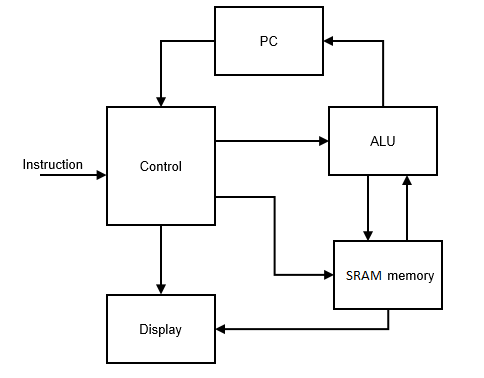
\includegraphics[width=100mm]{Lab5/figures/block.png}
	\caption{Block overview of processor}
	\label{fig:block}
\end{figure} 

	
\subsection{Pre-lab}

Before coming to the lab, please complete the following and upload to Sakai:
\begin{itemize}
	\item Read through the lab handout (especially Section \ref{sec:control}) and construct a top level finite state machine transition graph for the processor. Note that the different states are already defined in Section \ref{sec:control}.

	\item Read through the datasheet for working with the SRAM memory chip on the FPGA board. This can be found under Sakai Resources.
\end{itemize}

\subsection{Lab Activities}


\subsubsection{CPU Controller}
\label{sec:control}
Instructions are fed to the CPU controller as an 18 bit instruction IR, the format of an instruction can be seen in Table \ref{tab:instruct}. 

\begin{table}[H]
	\caption{18 bit instruction format}
	\label{tab:instruct}
	\begin{center}
		\begin{tabular}{| c | c | c | c |}
			\hline
			{\bf OPCODE} & {\bf Destination Address} & {\bf Source Address 1} & {\bf Source Address 2 / Shift Amount} \\ \hline
			3 bits & 5 bits & 5 bits & 5 bits \\ 
			\hline
		\end{tabular}
	\end{center}
\end{table}

The Control module should take apart the instruction IR and break it down into signals to be used by the other entities. It is best to think of Control as a "Top" level state machine for the entire processor. The processor should have the following states \emph{FETCH}, \emph{DECODE}, \emph{EXECUTE}, \emph{MEMORY\_WRITE}. Note that during each state, the display will show information relative to that state it is currently in, this explained in Section \ref{sec:display}. \\ 

The device should initiate in the \emph{FETCH} state by sending an active low RESET signal by pressing KEY(1) after startup. If RESET is HIGH, take in the instruction IR and proceed to the \emph{DECODE} state. \\

If the device is in the \emph{DECODE} state, you should break down the instruction IR into the various signals required for the entities ALU and SRAM. You should also read in the data stored from Source Address 1 and Source Address 2 and store it into a register. Once this is completed,  proceed to the \emph{EXECUTE} state. \\

In the \emph{EXECUTE} state, you should preform the ALU operation as determined from the processor instruction and store the result into a register. Once completed,  move to the next state \emph{MEMORY\_WRITE}. \\

After the instruction is completed, take the result and write it into the Destination Address on the SRAM memory. At this point you should increment the Program Counter and proceed back to \emph{FETCH} to begin working on the next instruction. \\

Each state should transition on the positive edge of a clock pulse which will come from pressing KEY0.

\subsubsection{Design an ALU}
Using the operations listed in Table \ref{tab:aluop}, create an ALU in VHDL that takes in two 8 bit values and returns the result to the processor. Required signals: {\bf A}, {\bf B}, {\bf opcode}, and {\bf ALU\_out}. Note that the inputs {\bf A} and {\bf B} should be read from the SRAM memory controller ,  {\bf ALU\_out} is an output register for the ALU  where the result of the operation will be stored prior to the \emph{MEMORY\_WRITE} state. {\bf OPCODE} comes from IR. Make sure to pay attention for converting A and B to either signed or unsigned to be able to perform certain operations.

\begin {table}[H]
	\caption {List of ALU operations} 
	\label{tab:aluop} 
	\begin{center}
    		\begin{tabular}{ | c | c |}
			\hline
 			{\bf OPCODE} & {\bf Instruction} \\ \hline
			000 & AND \\ \hline
			001 & OR \\ \hline
			010 & NAND \\ \hline
			011 & NOR \\ \hline
			100 & XOR \\ \hline
			101 & ADD \\ \hline
			110 & SUB \\ \hline
			111 & Shift Right Logical \\
			\hline
    		\end{tabular}
	\end{center}
\end{table}

\subsubsection{Initiate the SRAM}

Using the DE2-115 Control Panel, initiate arbitrary values into the SRAM and keep a record of this data to compare your results. Figure \ref{fig:controlpanel} shows the option screen for loading values. More information for this step will be provided in the lab.

\begin{figure}[H]
	\centering
	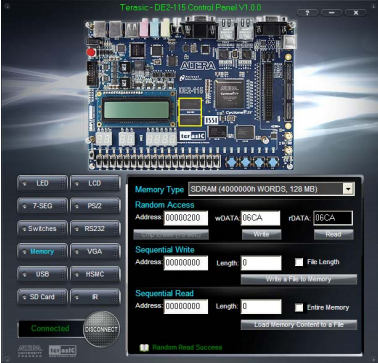
\includegraphics[width=100mm]{Lab5/figures/controlpanel.png}
	\caption{DE2-115 Control Panel - Accessing SRAM/SDRAM/FLASH/EEPROM Menu}
	\label{fig:controlpanel}
\end{figure}

\subsubsection{SRAM Memory Controller}
The Altera DE2-115 FPGA Development Board contains an 2 MB SRAM memory chip. For this component of the lab you will utilize the Altera SRAM IP to interface with the SRAM memory chip. A list of pins used for interacting with the chip can be found in Table \ref{tab:sram}. Notice that addresses are normally 20 bits long, however for this exercise you should set SRAM\_ADDR[0]  to SRAM\_ADDR[4] to the source address and set the remaining bits to zero. 

The Altera SRAM IP provides flags for enabling or disabling the SRAM read and write functions. Make sure that if read is HIGH then write should be LOW and vice versa. The clock signal for the SRAM should come from CLOCK\_50 a signal attached to the 50Mhz oscillator on the FPGA board.

Keep in mind that SRAM is volatile memory which means that when power is disconnected from the board, all data stored will be lost. 

\begin {table}[H]
	\caption {Signal assignments for interfacing with the SRAM memory chip} 
	\label{tab:sram} 
	\begin{center}
    		\begin{tabular}{ | c | c | c |}
			\hline
 			{\bf Signal} & {\bf Data Direction} & {\bf Description}  \\ \hline
			SRAM\_ADDR[0] to SRAM\_ADDR[19] & OUT &  SRAM Address[0] to SRAM Address[22] \\ \hline
			SRAM\_DQ[0] to SRAM\_DQ[15] & INOUT & SRAM Data[0] to SRAM Data[15] \\ \hline
			SRAM\_CE\_N & BUFFER & Active low SRAM Chip Enable \\ \hline
			SRAM\_OE\_N & BUFFER & Active low SRAM Output Enable \\ \hline
			SRAM\_WE\_N & BUFFER & Active low SRAM Write Enable \\ \hline
			SRAM\_LB\_N & BUFFER & Active low SRAM Lower Byte Strobe \\ \hline
			SRAM\_UB\_N & BUFFER & Active low SRAM Upper Byte Strobe \\ 
			\hline
    		\end{tabular}
	\end{center}
\end{table}

\subsubsection{Program Counter}

Design a simple program counter that keeps track of the number of operations completed and increments by one at the end of MEMORY\_WRITE. Store the result to a register to be shown through the display driver. Suggested signals to use are increment\_flag, current\_count, and prev\_count.

\subsubsection{Results Display}
\label{sec:display}
As has been done in previous labs, create a display driver for showing information relative the the current state.

\begin{enumerate}
	\item LEDG3 through LEDG0 should display the current state; FETCH, DECODE, EXECUTE, and MEMORY\_WRITE respectively. 
	\item \emph{FETCH}
	\begin{itemize}
		 \item Display a dash "-" across all displays.
	\end{itemize}
	\item \emph{DECODE}
	\begin{itemize}
		\item HEX7 and HEX6 should display the Source Address 1 from IR.
		\item HEX5 and HEX4 should display the Source Address 2 from IR.
		\item HEX3 should display the ALU operation from IR.
		\item HEX0 should display the current Program Counter.
	\end{itemize}
	\item \emph{EXECUTE}
	\begin{itemize}
		\item HEX7 and HEX6 should display the value stored in Source Address 1.
		\item HEX5 and HEX4 should display the value stored in Source Address 2.
		\item HEX3 and HEX2 should display ALU\_out the result of the operation.
		\item HEX0 should display the current Program Counter.
	\end{itemize}
	\item \emph{MEMORY\_WRITE}
	\begin{itemize}
		\item HEX7 and HEX6 should display the Destination Address.
		\item HEX3 and HEX2 should display the value stored in the Destination Address.
		\item HEX0 should display the incremented Program Counter.
	\end{itemize}
\end{enumerate}

\subsection{Lab Report}
After completing the activities in this lab you should complete the following and then submit it to Sakai:

\begin{itemize}

	\item Extract from the fpga lab folder the VHDL file from the project and upload it to the Sakai Assignment page. Ex: part1.vhd

	\begin{itemize}

		\item Make sure that your code is well commented.

	\end{itemize}

	\item Take a photo of each operation during the EXECUTE state, insert them into a document and include a note under each and explain the operation being performed.

	\item This processor is single-cycle which means it can only run one instruction at a time, how would you make the processor run in parallel? How many instructions can theoretically be worked on at the same time? Provide a diagram along with a short written response.

	\item Feedback on this lab course including what you enjoyed and what you did not like. Propose possible changes for the future and include whether the lab as a whole met your expectations. Would you recommend this lab to a friend?
\end{itemize}